\documentclass{article} % A4 paper and 11pt font size
\setcounter{secnumdepth}{0}

\usepackage{amssymb, amsmath, amsfonts}
\usepackage{moreverb}
\usepackage{graphicx}
\usepackage{enumerate}
\usepackage{graphics}
\usepackage[margin=1.25in]{geometry}
\usepackage{color}
\usepackage{tocloft}
\renewcommand{\cftsecleader}{\cftdotfill{\cftdotsep}}
\usepackage{array}
\usepackage{float}
\usepackage{hyperref}
\usepackage{textcomp}
\usepackage[makeroom]{cancel}
\usepackage{bbold}
\usepackage{alltt}
\usepackage{physics}
\usepackage{mathtools}
\usepackage{amsthm}
\usepackage{tikz}
\usetikzlibrary{positioning}
\usetikzlibrary{arrows}
\usepackage{pgfplots}
\usepackage{bigints}
\allowdisplaybreaks
\pgfplotsset{compat=1.12}

\theoremstyle{plain}
\newtheorem*{theorem*}{Theorem}
\newtheorem{theorem}{Theorem}
\newtheorem*{lemma*}{Lemma}
\newtheorem{lemma}{Lemma}

\newenvironment{definition}[1][Definition]{\begin{trivlist}
\item[\hskip \labelsep {\bfseries #1}]}{\end{trivlist}}

\newcommand{\E}{\varepsilon}
\def\Rl{\mathbb{R}}
\def\Cx{\mathbb{C}}

\usepackage[T1]{fontenc} % Use 8-bit encoding that has 256 glyphs
\usepackage{fourier} % Use the Adobe Utopia font for the document - comment this line to return to the LaTeX default
\usepackage[english]{babel} % English language/hyphenation

\usepackage{sectsty} % Allows customizing section commands
\allsectionsfont{\centering \normalfont\scshape} % Make all sections centered, the default font and small caps

\usepackage{fancyhdr} % Custom headers and footers
\pagestyle{fancy} % Makes all pages in the document conform to the custom headers and footers
\fancyhead[L]{\bf Sam Fleischer}
\fancyhead[C]{\bf UC Davis \\ Applied Mathematics (MAT207B)} % No page header - if you want one, create it in the same way as the footers below
\fancyhead[R]{\bf Winter 2016}

\fancyfoot[L]{\bf } % Empty left footer
\fancyfoot[C]{\bf \thepage} % Empty center footer
\fancyfoot[R]{\bf } % Page numbering for right footer
\renewcommand{\headrulewidth}{0pt} % Remove header underlines
\renewcommand{\footrulewidth}{0pt} % Remove footer underlines
\setlength{\headheight}{25pt} % Customize the height of the header

\newcommand{\problem}[1]{
\vspace{.375cm}
\begin{minipage}{\textwidth}
    \begin{center}
        \noindent\rule{5cm}{1pt}
    \end{center}
    \section{\bf #1}
    \begin{center}
        \noindent\rule{5cm}{1pt}
    \end{center}
    \vspace{0.25cm}
\end{minipage}
}

\newcommand{\VEC}[2]{\left\langle #1, #2 \right\rangle}

% \numberwithin{equation}{section} % Number equations within sections (i.e. 1.1, 1.2, 2.1, 2.2 instead of 1, 2, 3, 4)
% \numberwithin{figure}{section} % Number figures within sections (i.e. 1.1, 1.2, 2.1, 2.2 instead of 1, 2, 3, 4)
% \numberwithin{table}{section} % Number tables within sections (i.e. 1.1, 1.2, 2.1, 2.2 instead of 1, 2, 3, 4)

\setlength\parindent{0pt} % Removes all indentation from paragraphs - comment this line for an assignment with lots of text

\newcommand{\horrule}[1]{\rule{\linewidth}{#1}} % Create horizontal rule command with 1 argument of height

\title{ 
\normalfont \normalsize 
\textsc{UC Davis, Applied Mathematics (MAT207B), Winter 2016} \\ [25pt] % Your university, school and/or department name(s)
\horrule{2pt} \\[0.4cm] % Thin top horizontal rule
\Huge Homework \#5 \\ % The assignment title
\horrule{2pt} \\[0.5cm] % Thick bottom horizontal rule
}

\author{\huge Sam Fleischer} % Your name

\date{February 19, 2016} % Today's date or a custom date

\begin{document}\thispagestyle{empty}

\maketitle % Print the title

\makeatletter
\@starttoc{toc}
\makeatother

\pagebreak
\problem{Problem 1}
\emph{Suppose that $p\ :\ [a,b]\rightarrow \Rl$ is a continuously differentiable function such that $p > 0$ and $q,r\ :\ [a,b]$ are continuous functions such that $r > 0$, $q \geq 0$.  Define a weighted inner product on $L^2(a,b)$ by $$\VEC{u}{v}_r = \int_a^b r(x) \overline{u(x)}v(x) \dd x.$$  Let $A\ :\ D(A) \subset L^2(a,b) \rightarrow L^2(a,b)$ by $$A = \frac{1}{r(x)}\qty[-\frac{\dd}{\dd x}p(x) \frac{\dd}{\dd x} + q(x)]$$ with Dirichlet boundary conditions and domain $$D(A) = \left\{u \in H^2(a,b)\ :\ u(a) = 0 = u(b)\right\}.$$}
\begin{enumerate}[\bf (a)]
    \item
        \emph{Show that $$\VEC{u}{Av}_r = \VEC{Au}{v}_r \qquad \text{for all } u, v \in D(A),$$ meaning that $A$ is self-adjoint with respect to $\VEC{\cdot}{\cdot}_r$.} \\

        Denote the real and complex parts of a function $u$ by $u_r$ and $u_i$, respectively.  Then
        \begin{align*}
            \VEC{u}{Av}_r &= \int_a^b r\overline{u}\frac{1}{r}\qty[-(pv')' + qv]\dd x \\
            &= \int_a^b ru_r\frac{1}{r}\qty[-(pv')' + qv]\dd x  - i\int_a^b ru_i\frac{1}{r}\qty[-(pv')' + qv]\dd x \\
            &= \int_a^b u_r\qty[-(pv')' + qv]\dd x  - i\int_a^b u_i\qty[-(pv')' + qv]\dd x
        \end{align*}
        By Homework 4 number 3,
        \begin{align*}
            \VEC{u}{Av}_r &= \qty[p\qty((u_r'v - u_rv') - i(u_i'v - u_iv'))]_a^b + \VEC{rAu_r}{v} - i\VEC{rAu_i}{v}
        \end{align*}
        where $\VEC{u}{v}$ is the unweighted innerproduct of $u$ and $v$.  The Dirichlet boundary condition $u(a) = u(b) = 0$ implies $u_r(a) = u_r(b) = u_i(a) = u_i(b) = 0$.  If we assume the adjoint boundary condition on $v$,
        \begin{align*}
            v_r(a) = v_r(b) = v_i(a) = v_i(b) = 0
        \end{align*}
        then
        \begin{align*}
            \VEC{u}{Av}_r = \VEC{rAu_r}{v} - i\VEC{rAu_i}{v} = \VEC{rAu}{v}
        \end{align*}
        since inner products are conjugate-linear in the first term.  However, since $r > 0$, then
        \begin{align*}
            \VEC{ru}{v} = \int_a^b\overline{ru}v\dd x = \int_a^b r\overline{u}v\dd x = \VEC{u}{v}_r
        \end{align*}
        which proves
        \begin{align*}
            \VEC{u}{Av}_r = \VEC{rAu}{v} = \VEC{Au}{v}_r
        \end{align*}
        Thus, $A$ is self-adjoint with respect to $\VEC{\cdot}{\cdot}_r$.
    \item
        \emph{Show that the eigenvalues $\lambda$ of the weighted Sturm-Liouville eigenvalue problem $$-\qty(pu')' + qu = \lambda r u, \qquad u(a) = 0 = u(b)$$ are real and positive and eigenfunctions associated with different eigenvalues are orthogonal with respect to $\VEC{\cdot}{\cdot}_r$.} \\

        Eigenvalues $\lambda$ of $-\qty(pu')' + qu = \lambda r u$; $u(a) = 0 = u(b)$ are eigenvalues of
        \begin{align*}
            A u = \lambda u, \qquad u(a) = 0 = u(b)
        \end{align*}
        where $A$ is defined above.  We showed $A$ is self-adjoint with respect to $\VEC{\cdot}{\cdot}_r$ in part \textbf{(a)}.  Thus if $Au = \lambda u$,
        \begin{align*}
            \VEC{Au}{u}_r = \VEC{\lambda u}{u}_r = \overline{\lambda}\VEC{u}{u}_r \qquad \text{and} \qquad \VEC{u}{Au}_r = \VEC{u}{\lambda u}_r = \lambda\VEC{u}{u}_r
        \end{align*}
        Thus $\lambda = \overline{\lambda}$ or $u = 0$, i.e. $\lambda \in \Rl$ if $\lambda$ is an eigenvalue.  Note
        \begin{align*}
            \lambda = \frac{\VEC{u}{Au}_r}{\VEC{u}{u}_r}
        \end{align*}
        implies $\lambda > 0$ since $u \neq 0$ and inner-products are positive-definite.

        Now consider eigenfunctions of $A$, $\phi_n$, $\phi_m$ with eigenvalues $\lambda_n$ and $\lambda_m$, respectively ($\lambda_n \neq \lambda_m$).  Then
        \begin{align*}
            A\phi_n = \lambda_n \phi_n \qquad \text{and} \qquad A\phi_m = \lambda_m \phi_m
        \end{align*}
        By multiplying the left equation by $\phi_m$ and the right equation by $\phi_n$, and subtracting the two equations, we see
        \begin{align*}
            \phi_m A\phi_n - \phi_n A\phi_m = \qty(\lambda_n - \lambda_m)\phi_n\phi_m \\
            \implies \VEC{\phi_m}{A\phi_n}_r - \VEC{A\phi_m}{\phi_n}_r = \int_a^b \qty(\lambda_n - \lambda_m)\phi_n\phi_m \dd x
        \end{align*}
        Then since $A$ is self-adjoint,
        \begin{align*}
            0 = \frac{1}{r}0 = (\lambda_n - \lambda_m)\int_a^b \phi_n\phi_m \dd x \\
            \implies 0 &= \int_a^b\phi_n\phi_mr \dd x \\
            &= \VEC{\phi_n}{\phi_m}_r
        \end{align*}
        and thus $\phi_n$ and $\phi_m$ are orthogonal.
\end{enumerate}
\problem{Problem 2}
\emph{A nonuniform string of length one with wave speed $c_0(x) = \sqrt{\dfrac{T}{\rho_0(x)}} > 0$ is fixed at each end, with zero initial displacement and nonzero initial velocity.  The transverse displaceent $y = u(x,t)$ of the string satisfies the IBVP}
\begin{align*}
    \begin{array}{lll}
        u_{tt} = c_0^2(x)u_{xx}, & 0 < x < 1, & t > 0, \\
        u(0, t) = 0, & u(1,t) = 0, & t > 0, \\
        u(x,0) = 0, & 0 < x < 1, & \\
        u_t(x,0) = g(x), & 0 < x < 1, &
    \end{array}
\end{align*}
\emph{Find the solution in terms of the eigenvalues $\lambda_n$ and eigenfunctions $\phi_n(x)$ of the weighted Sturm-Liouville problem $$-c_0^2\phi_n'' = \lambda_n\phi_n, \qquad \phi_n(0) = 0, \qquad \phi_n(1) = 0, \qquad n = 1, 2, 3, \dots$$}

Suppose $u(x,t) = F(x)G(t)$.  Then
\begin{align*}
    F(x)G''(t) &= c_0^2(x)F''(x)G(t) \\
    \qty(\frac{G''}{G})(t) &= \qty(\frac{F''c_0^2}{F})(x) = -\lambda \in \Rl
\end{align*}
since the left hand side is a function of $t$ and the right hand side is a function of $x$.  Then
\begin{align*}
    -c_0^2(x)F''(x) = \lambda F(x)
\end{align*}
By Problem 1 ($p \equiv 1$, $q \equiv 0$, and $r \equiv \frac{1}{c_0^2}$) this implies the eigenfunctions $\phi_n(x)$ are orthogonal and its eigenvalues $\lambda_n$ are real and $\lambda_n > 0$ for all $n$.  Then
\begin{align*}
    G'' &= -\lambda G \qquad \lambda > 0 \\
    \implies G(t) &= \sum_{n=1}^\infty \qty[a_n\cos\qty(\sqrt{\lambda_n}t) + b_n\sin\qty(\sqrt{\lambda_n}t)] \\
    \implies u(x,t) &= \sum_{n=1}^\infty \left\{\qty[a_n\cos\qty(\sqrt{\lambda_n}t) + b_n\sin\qty(\sqrt{\lambda_n}t)]\phi_n(x)\right\} \\
    \implies 0 = u(x,0) &= \sum_{n=1}^\infty \qty[a_n\phi_n(x)] \\
    \implies a_n &= 0 \text{ for } n = 1, 2, \dots \qquad \text{because $\{\phi_n\}_n$ is a linearly independent set} \\
    \implies u(x,t) &= \sum_{n=1}^\infty \left\{\qty[b_n\sin\qty(\sqrt{\lambda_n}t)]\phi_n(x)\right\} \\
    \implies u_t(x,t) &= \sum_{n=1}^\infty \left\{\sqrt{\lambda_n}b_n\cos\qty(\sqrt{\lambda_n}t)\phi_n(x)\right\} \\
    \implies g(x) = u_t(x,0) &= \sum_{n=1}^\infty \qty[\sqrt{\lambda_n}b_n\phi_n(x)]
\end{align*}
Thus the coefficients $\sqrt{\lambda_n}b_n$ are Fourier coefficients with respect to the weighted norm $\VEC{\cdot}{\cdot}_{c_0^2}$, i.e.
\begin{align*}
    \sqrt{\lambda_n}b_n = \VEC{g(x)}{\phi_n(x)}_{c_0^2(x)}
\end{align*}
So,
\begin{align*}
    u_t(x,t) &= \sum_{n=1}^\infty \left\{\VEC{g(x)}{\phi_n(x)}_{c_0^2(x)}\cos\qty(\sqrt{\lambda_n}t)\phi_n(x)\right\}
\end{align*}

\problem{Problem 3}
\emph{The Fourier solution of the initial value problem}
\begin{align*}
    &\begin{array}{lll}
        u_{tt} = u_{xx}, &0 < x < 1, & t > 0, \\
        u(0, t) = 0, & u(1, t) = 0, & t > 0
    \end{array} \\
    &u(x,0) = \begin{cases}
        2x & \text{ if } 0 \leq x \leq \frac{1}{2} \\
        2(1-x) & \text{ if } \frac{1}{2} < x < 1
    \end{cases}, \\
    &= u_t(x,0) = 0, \qquad 0 \leq x \leq 1
\end{align*}
\emph{is given by $$u(x,t) = \frac{8}{\pi^2}\sum_{n=1}^\infty \frac{(-1)^{n+1}}{(2n-1)^2}\sin\qty[(2n-1)\pi x]\cos\qty[(2n-1)\pi t]$$}
\begin{enumerate}[\bf (a)]
    \item
        \emph{Show that the Fourier seires converges to a continuous function.  How many spacial (weak) $L^2$-derivatives does $u(x,t)$ have?} \\

        For a fixed $t$, it suffices to show the partial sums $u_N$ converge to a function in $H^k$ for $k < \frac{3}{2}$ (and $u \not\in H^k$ for $k \geq \frac{3}{2}$) where $H^k$ is the Sobolev space of order $k$.  Then by the Sobolev Embedding Theorem, $u$ converges to a continuous function.  Thus, that continuous function has a weak spacial $L^2$ derivative $u' \not\in H^{\frac{1}{2}}$, and so $u$ does not have two weak spacial derivatives.

        To show this is true, fix $t$ and denote $c_t = \cos\qty[\qty(2n-1)\pi t] \in \Rl$.  Then the Fourier coefficients $\hat{u}_n$ are proportional to the following (we do not say equal since we want to consider the standard Fourier basis $\left\{e^{inx}\right\}_{n\in\mathbb{Z}}$ as opposed to the basis $\big\{1, \sin nx, \cos nx\big\}_{n=1}^\infty$).
        \begin{align*}
            \left|\hat{u}_n\right| \propto \frac{1}{(2n-1)^2} \qquad \text{and} \qquad \sum_{n=1}^\infty \hat{u}_n^2 \propto \sum_{n=1}^\infty \frac{1}{n^4}
        \end{align*}
        which converges.  Then the Fourier coefficients of the weak derivative are proportional to the following:
        \begin{align*}
            \left|\hat{u'}_n\right| = \left|n\hat{u}_n\right| \propto \frac{n}{(2n-1)^2} \qquad \text{and} \qquad \sum_{n=1}^\infty \hat{u'}_n^2 \propto \sum_{n=1}^\infty \frac{1}{n^2}
        \end{align*}
        which also conveges.  However,
        \begin{align*}
            \left|\hat{u''}_n\right| = \left|n^2\hat{u}_n\right| \propto \frac{n^2}{(2n-1)^2} \qquad \text{and} \qquad \sum_{n=1}^\infty \hat{u''}_n^2 \propto \sum_{n=1}^\infty 1
        \end{align*}
        which diverges.
    \item
        \emph{Verify from the Fourier solution that $$\int_0^1\qty[u_t^2(x,t) + u_x^2(x,t)]\dd x = \text{constant} \qquad \text{ for } -\infty < t < \infty.$$}

        First note
        \begin{align*}
            u_x(x,t) = \frac{8}{\pi^2}\sum_{n=1}^\infty \frac{(-1)^{n+1}}{(2n-1)^2}(2n-1)\pi\cos\qty((2n-1)\pi x)\cos\qty((2n-1)\pi t), \qquad \text{and} \\
            u_t(x,t) = \frac{8}{\pi^2}\sum_{n=1}^\infty \frac{(-1)^n}{(2n-1)^2}(2n-1)\pi\sin\qty((2n-1)\pi x)\sin\qty((2n-1)\pi t)
        \end{align*}
        and since
        \begin{align*}
            \int_0^1 \cos((2n-1)\pi x)\cos((2m-1)\pi x)\dd x = \int_0^1 \sin((2n-1)\pi x)\sin((2m-1)\pi x)\dd x = \frac{1}{2}\delta_{n,m} = \begin{cases}
                \frac{1}{2} & \text{ if } n = m\\
                0 & \text{ if } n \neq m
            \end{cases}
        \end{align*}
        then
        \begin{align*}
            \int_0^1 u_t^2 \dd x &= \frac{64}{\pi^2}\sum_{n=1}^\infty \frac{1}{(2n-1)^2}\sin^2((2n-1)\pi t)\int_0^1\sin^2((2n-1)\pi x)\dd x, \qquad \text{and} \\
            \int_0^1 u_x^2 \dd x &= \frac{64}{\pi^2}\sum_{n=1}^\infty \frac{1}{(2n-1)^2}\cos^2((2n-1)\pi t)\int_0^1\cos^2((2n-1)\pi x)\dd x \\
            \implies \int_0^1 \qty[u_t^2 + u_x^2]\dd x & \\
            = \frac{64}{\pi^2}\sum_{n=1}^\infty \frac{1}{(2n-1)^2}&\qty[\sin^2((2n-1)\pi t)\int_0^1 \sin^2((2n-1)\pi x)\dd x + \cos^2((2n-1)\pi t)\int_0^1 \cos^2((2n-1) \pi x)\dd x] \\
            &= \frac{32}{\pi^2}\sum_{n=1}^\infty \frac{1}{(2n-1)^2}\qty[\sin^2((2n-1)\pi t) + \cos^2((2n-1)\pi t)] \\
            &= \frac{32}{\pi^2}\sum_{n=1}^\infty \frac{1}{(2n-1)^2} \\
            &= \frac{32}{\pi^2}\cdot\frac{\pi^2}{8} \\
            &= 4
        \end{align*}
    \item
        \emph{Use \texttt{MATLAB} (or another program) to compute the partial sum $$u_N(x,t) = \frac{8}{\pi^2}\sum_{n=1}^N\frac{(-1)^{n+1}}{(2n-1)^2}\sin\qty[(2n-1)\pi x]\cos\qty[(2n-1)\pi t]$$ at $t = 0.25$ for $N = 5$ and $N = 50$.}
        \begin{center}
            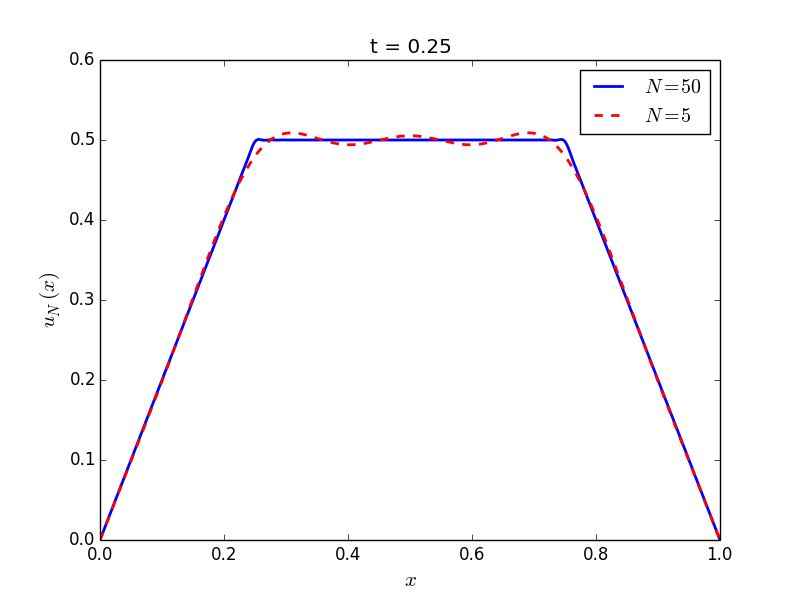
\includegraphics[scale=0.75]{problem_3c.png}
        \end{center}
    \item
        \emph{Use the addition formula for sines to show that the Fourier solution can be written in the form of the d'Alembert solution as $$u(x,t) = F(x - t) + F(x + t)$$ for a suitable function $F\ :\ \Rl \rightarrow \Rl$.  What is $F$?} \\

        Define $\tilde{F}$ as half the initial data, i.e.
        \begin{align*}
            \tilde{F}(x) = \begin{cases}
                x & \text{ if } 0 \leq x \leq n + \frac{1}{2} \\
                1 - x & \text{ if } \frac{1}{2} < x < 1
            \end{cases}
        \end{align*}
        Let $F$ be it's odd $2$-periodic expansion,
        \begin{align*}
            F(x) = \begin{cases}
                x & \text{ if } n - \frac{1}{2} \leq x \leq n + \frac{1}{2} \\
                1 - x & \text{ if } n + \frac{1}{2} < x < n + \frac{3}{2}
            \end{cases} \qquad \frac{n}{2} \in \mathbb{Z}
        \end{align*}
        and note its Fourier series representation:
        \begin{align*}
            F(x) = \frac{4}{\pi^2}\sum_{n=1}^\infty \frac{(-1)^{n+1}}{(2n-1)^2}\sin((2n-1)\pi x)
        \end{align*}
        Then note $F(x - t) + F(x + t) = u(x,t)$ because
        \begin{align*}
            F(x - t) + F(x + t) &= \frac{4}{\pi^2}\sum_{n=1}^\infty \frac{(-1)^{n+1}}{(2n-1)^2}\sin((2n-1)\pi (x - t)) + \frac{4}{\pi^2}\sum_{n=1}^\infty \frac{(-1)^{n+1}}{(2n-1)^2}\sin((2n-1)\pi (x + t)) \\
            &= \frac{8}{\pi^2}\sum_{n=1}^\infty \frac{(-1)^{n+1}}{(2n-1)^2}\frac{1}{2}\qty[\sin((2n-1)\pi(x-t)) + \sin((2n-1)\pi(x+t))] \\
            &= \frac{8}{\pi^2}\sum_{n=1}^\infty \frac{(-1)^{n+1}}{(2n-1)^2}\sin((2n-1)\pi x)\cos((2n-1)\pi t) \\
            &= u(x,t)
        \end{align*}
\end{enumerate}
\problem{Problem 4}
\emph{Suppose that $u(x,t)$ is a smooth solution of the wave equation $$u_{tt} = c_0^2 \Delta u,$$ where $x \in \Rl^n$, the wave speed $c_0 > 0$ is a constant.}
\begin{enumerate}[\bf (a)]
    \item
        \emph{Show that $u$ satisfies the energy equation $$\frac{1}{2}\qty(u_t^2 + c_0^2|\grad u|^2)_t - \grad \cdot \qty(c_0^2 u_t\grad u) = 0.$$}
        \begin{align*}
            u_{tt} &= c_0^2 \Delta u \\
            \iff u_tu_{tt} &= c_0^2 u_t\Delta u \\
            \iff u_tu_{tt} + c_0^2 \grad u \cdot \grad u_t &= c_0^2u_t\Delta u + c_0^2 \grad u \cdot \grad u_t \\
            \iff \frac{1}{2}\qty(u_t^2 + c_0^2|\grad u|^2)_t &= \grad \cdot \qty(c_0^2 u_t \grad u)
        \end{align*}
    \item
        \emph{For $T > 0$, let $\Omega_T \subset \Rl^{n+1}$ be the space-time cone $$\Omega_T = \left\{(x,t) \in \Rl^{n+1}\ :\ |x| < c_0(T - t),\ 0 < t < T\right\},$$ and for $0 \leq t \leq T$, let $B(T - t)$ be the spatial cross-section of $\Omega_T$ at time $t$ $$B(T - t) = \left\{x \in \Rl^n\ :\ |x| < c_0(T - t)\right\}.$$  Define $$e_T(t) = \frac{1}{2}\int_{B(T - t)}\qty(u_t^2 + c_0^2|\grad u|^2)\dd x,$$ and show that $e_T(t) \leq e_T(0)$.}

        \emph{HINT.  Apply the divergence theorem in space-time to the equation in \textbf{(a)} over the truncated cone $\left\{(x, t') \in \Omega_T\ :\ 0 < t' < t\right\}$, and note that the space-time normal to the side of the cone $\Omega_T$ is $N = \dfrac{(\hat{x}, c_0)}{\sqrt{1 + c_0^2}}$ where $\hat{x} = \dfrac{x}{|x|}$.} \\

        Let $F\ :\ \Rl^{n+1} \rightarrow \Rl^{n+1}$ by
        \begin{align*}
            F(\vec{x}, t) &= \VEC{-c_0^2 u_t \grad u}{\frac{1}{2}\qty(u_t^2 + c_0^2\left|\grad u\right|^2)} \\
            \implies \grad \cdot F &= \qty(-c_0^2 u_t \grad u)_{\vec{x}} + \frac{1}{2}\qty(u_t + c_0^2 + \left|\grad u\right|^2)_t \\
            &= \grad\qty(-c_0^2 u_t \grad u) + \frac{1}{2}\qty(u_t + c_0^2 + \left|\grad u\right|^2)_t
        \end{align*}
        For ease, denote $\Omega_{T, t}$ to be the truncated cone, i.e.
        \begin{align*}
            \Omega_{T, t} = \left\{(x, t') \in \Omega_T\ :\ 0 < t' < t\right\}
        \end{align*}
        and denote the curved ``side'' part of the boundary of the cone as
        \begin{align*}
            \partial\Omega_{T, t, \text{side}} = \left\{x \in \partial\Omega_{T, t}\ :\ \vec{n} \neq (0, 1) \text{ or } \vec{n} \neq (0, -1) \right\}
        \end{align*}
        Thus by the divergence theorem,
        \begin{align*}
            0 &= \int_{\Omega_{T, t}} \grad \cdot F \dd V \\
            &= \int_{\partial \Omega_{T, t}} F \cdot \vec{n} \dd s \\
            &= \int_{B(T)} F \cdot \VEC{0}{-1} \dd s + \int_{B(T-t)} F \cdot \VEC{0}{1} \dd s + \int_{\partial \Omega_{T, t, \text{side}}} F \cdot \frac{\VEC{\hat{x}}{c_0}}{\sqrt{1 + c_0^2}}\dd s\\
            &= -e_T(0) + e_T(t) + \int_{\partial \Omega_{T, t, \text{side}}} \qty[\cancelto{0}{-\frac{c_0^2 u_t \grad u \hat{x}}{\sqrt{1 + c_0^2}}} + \frac{\frac{1}{2}\qty(u_t^2 + c_0^2\left|\grad u\right|^2)c_0}{\sqrt{1 + c_0^2}}]\dd s
        \end{align*}
        Since the integrand is always positive, then
        \begin{align*}
            0 \leq e_T(t) \leq e_T(0)
        \end{align*}
    \item
        \emph{Suppose that $u_1, u_2$ are smooth solutions of the wave equation such that $$u_i(x,0) = f_i(x), \qquad u_{it}(x,0) = g_i(x), \qquad i = 1, 2$$ where $f_i = g_i$ in $|x| \leq c_0 T$.  Show that $u_1 = u_2 \in \Omega_T$.}

        \emph{HINT.  Consider $u = u_1 - u_2$.} \\

        Let $u = u_1 - u_2$.  Then since $u$ is a linear combination of solutions of the wave equation then $u$ is a solution of the wave equation.  Then note $u(x,0) = u_1(x,0) - u_2(x,0) = 0$ and $u_t(x,0) = u_{1t}(x,0) - u_{2t}(x,0) = 0$.  Also, since $u$ is sufficiently smooth, then
        \begin{align*}
            (\grad u)(x,0) = \grad(u(x,0)) = \grad 0 = 0
        \end{align*}
        for all $x$.  Then fix $t \in [0, T]$ and note that by part \textbf{(b)},
        \begin{align*}
            0 \leq e_T(t) \leq e_T(0) = \int_{B(T)}\qty[u_t^2(x,0) + c_0^2|\grad u(x,0)|^2]\dd x
        \end{align*}
        However, initial conditions $u_t(x,0) = \grad u(x,0) = 0$, and so
        \begin{align*}
            0 \leq e_T(t) \leq \int_B(T) \qty[\cancelto{0}{u_t^2(x,0)} + c_0^2\cancelto{0}{|\grad u (x,0)|^2}] = 0 \\
            \implies e_T(t) = 0 \qquad \forall t \in [0,T].
        \end{align*}
        Since $u_t^2 \geq 0$ and $|\grad u|^2 \geq 0$, then $u_t = 0$ and $\grad u = 0$ for all $t \in [0, T]$.  This shows $u$ is constant, i.e.
        \begin{align*}
            u(x,t) = K \in \mathbb{R}
        \end{align*}
        but $u(x,0) = 0 \implies K = 0$, i.e.~$u \equiv 0$, or
        \begin{align*}
            u_1 = u_2.
        \end{align*}
\end{enumerate}

\end{document}
